% Created 2013-10-20 Sun 13:48
\documentclass[11pt]{article}
\usepackage[latin1]{inputenc}
\usepackage[T1]{fontenc}
\usepackage{fixltx2e}
\usepackage{graphicx}
\usepackage{longtable}
\usepackage{float}
\usepackage{wrapfig}
\usepackage{soul}
\usepackage{textcomp}
\usepackage{marvosym}
\usepackage{wasysym}
\usepackage{latexsym}
\usepackage{amssymb}
\usepackage{hyperref}
\tolerance=1000
\providecommand{\alert}[1]{\textbf{#1}}

\title{BCNotes.org}
\author{Jim Durant}
\date{2013-10-01 Tue}
\hypersetup{
  pdfkeywords={},
  pdfsubject={},
  pdfcreator={Emacs Org-mode version 7.9.3f}}

\begin{document}

\maketitle

\setcounter{tocdepth}{3}
\tableofcontents
\vspace*{1cm}
\hrule
\section{Week 1 Notes}
\label{sec-1}
\subsection{Hypothesis Tests}
\label{sec-1-1}
\subsubsection{Standard Normal R Code}
\label{sec-1-1-1}


\begin{verbatim}
qnorm(.95)


xval <- seq(-3.2, 3.2, length = 1000)
yval<- dnorm(xval)

plot(xval, yval, type = "l", axes = TRUE, frame = FALSE, lwd = 3, xlab = "", ylab = "")
x <- seq(qnorm(.95), 3.2, length = 100)
polygon(c(x, rev(x)),c(dnorm(x), rep(0, length(x))), col = "salmon")
text(mean(x), mean(dnorm(x))+.02, "5%", cex = 2)
text(qnorm(.95), .01, "1.645", cex = 2)


plot(xval, yval, type = "l", axes = TRUE, frame = FALSE, lwd = 3, xlab = "", ylab = "")
x <- seq(qnorm(.975), 3.2, length = 100)
polygon(c(x, rev(x)),c(dnorm(x), rep(0, length(x))), col = "salmon")
text(mean(x), mean(dnorm(x))+.02, "2.5%", cex = 2)
text(qnorm(.975), .01, "1.96", cex = 2)
x <- seq(-3.2, qnorm(.025),length = 100)
polygon(c(x, rev(x)),c(dnorm(x), rep(0, length(x))), col = "salmon")
text(mean(x), mean(dnorm(x))+.02, "2.5%", cex = 2)
text(qnorm(.025), .01, "-1.96", cex = 2)
text(0, dnorm(0) / 5, "95%", cex = 2)
\end{verbatim}

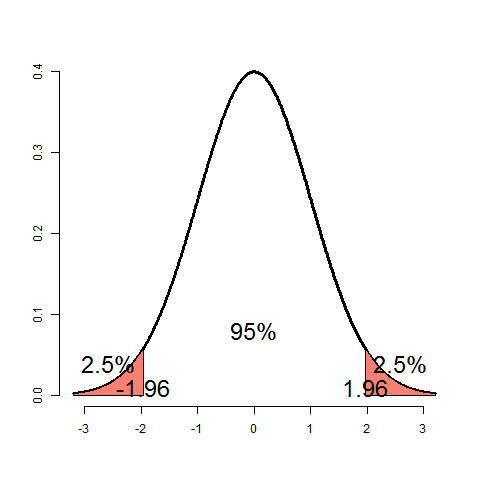
\includegraphics[width=.9\linewidth]{figure1.png}
\subsubsection{General Rules of Hypothesis Tests}
\label{sec-1-1-2}

$$\frac{32-30}{10\sqrt{100}} \ge 1.645$$

\begin{itemize}
\item The $Z$ test for $H_0: /mu = /mu_0$ versus
\item H$_1$: $\mu <\mu_0$
\item H$_2$: $\mu \ne \mu_0$
\item H$_3$: $\mu > \mu_0$
\item Test statistic $TS = \frac{\bar{X} -\mu_0}{S/\sqrt{n}}$
\item Reject the null hypothesis when
\item $H_1 : TS \le -Z_{1-\alpha}$
\item $H_2: |TS| \ge Z_{1-\alpha/2}$
\item $H_3: TS \ge Z_{1-\alpha}$
\end{itemize}

We want an $\alpha$ percent chance of rejecting the null hypothesis
falsely. We look at $\alpha$/2 because we want an overall rate of 5\%.


\begin{verbatim}
xval <- seq(-4, 4, length = 1000)
yval<- dt(xval, 15)
plot(xval, yval, type = "l", axes = TRUE, frame = FALSE, lwd = 3, xlab = "", ylab = "")
x <- seq(qt(.975, 15), 4, length = 100)
polygon(c(x, rev(x)),c(dt(x, 15), rep(0, length(x))), col = "salmon")
text(mean(x), mean(dt(x, 15))+.02, "2.5%", cex = 2)
text(qt(.975, 15), .01, "2.13", cex = 2)
x <- seq(-4, qt(.025, 15),length = 100)
polygon(c(x, rev(x)),c(dt(x, 15), rep(0, length(x))), col = "salmon")
text(mean(x), mean(dt(x, 15))+.02, "2.5%", cex = 2)
text(qt(.025, 15), .01, "-2.13", cex = 2)
text(0, dt(0, 15) / 5, "95%", cex = 2)
\end{verbatim}

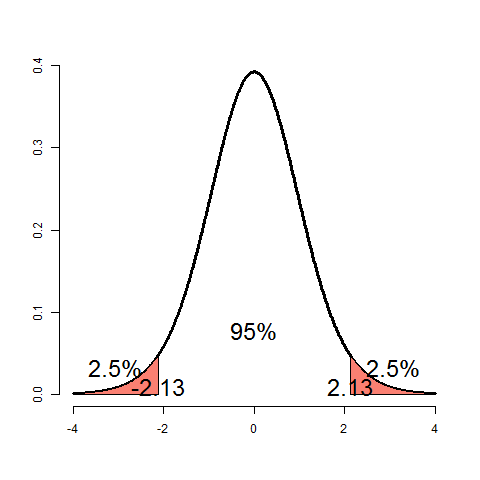
\includegraphics[width=.9\linewidth]{figure2.png}

Looking for greater than or less than critical values (overall rate
is 5\%)

We have forced the type I error rate to be small. We have not fixed
anything to do with the type II error. We say \emph{failed to reject H$_0$}
rather than accepting H$_0$. Small sample size can lead to variability
in the mean - we did not get enough data to reject. Classic phrase:
absence of evidence is not evidence of absence. \emph{Statistical significance is not scientific significance}. A big sample size may
lead to rejection of the null hypothesis - but the overall difference
is meaningless.
\begin{itemize}
\item The region of TS values for which you would reject the null is
  called the rejection region.

 *** Two sides tests
\item Z test required assumption of CLT
\item If n is small then a Gosset T test is performed
\item Power is used a lot to calculate sample sizes using guesses of
  standard errors and level of effect. This is done prior to
  experiment.
\item Consider example n=16 then:
\end{itemize}

Consider our example again. Suppose that $n= 16$ (rather than
$100$). Then consider that 
$$
.05 = P\left(\frac{\bar X - 30}{s / \sqrt{16}} \geq t_{1-\alpha, 15} ~|~ \mu = 30 \right)
$$
\begin{itemize}
\item s=10
\item n= 16
\item \bar{X} = 32
\end{itemize}
So that our test statistic is now $\sqrt{16}(32 - 30) / 10 = 0.8$, while the critical
value is $t_{1-\alpha, 15} = 1.75$. We now \underline{fail to reject}.

\emph{we went from 100 to 16} and the \emph{t-value went up} so we are not
surprised we did not reject.

\begin{itemize}
\item Suppose we want to test if $\mu \ne 30$ (does not make sense as we
  proposed the problem).
\item Then
\end{itemize}

$$\alpha = P\left(\left. \left|\frac{\bar X - 30}{s /\sqrt{16}}\right|
> t_{1-\alpha/2,15} ~\right|~ \mu = 30\right)$$

\begin{itemize}
\item we \underline{fail to reject} (0.8 < 2.13).
\end{itemize}


\begin{verbatim}
# add source code for t-tests. 

pt(.8, 15, lower.tail=FALSE)
xval <- seq(-4, 4, length = 1000)
yval<- dt(xval, 15)
plot(xval, yval, type = "l", axes = TRUE, frame = FALSE, lwd = 3, xlab = "", ylab = "")
x <- seq(.8, 4, length = 100)
polygon(c(x, rev(x)),c(dt(x, 15), rep(0, length(x))), col = "salmon")
text(mean(x), mean(dt(x, 15))+.02, "22%", cex = 2)
text(0.8, .01, "0.8", cex = 2)
\end{verbatim}

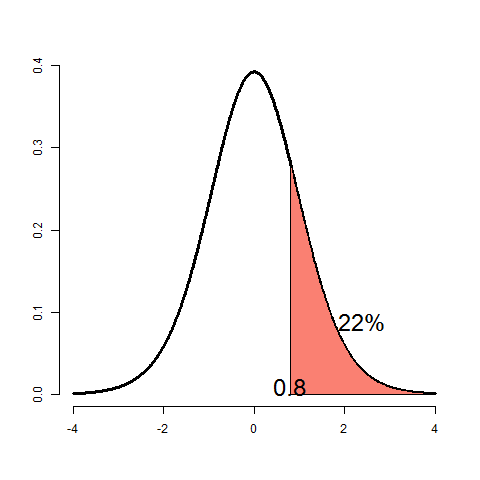
\includegraphics[width=.9\linewidth]{figure3.png}
\subsubsection{Connections with confidence intervals and P Values}
\label{sec-1-1-3}

\begin{itemize}
\item test H$_0$: $\mu$ = $\mu$$_0$ versus H$_a$: $\mu$ $\ne$ \m$_0$
\item range of possible values that we do not reject H$_0$ is confidence
  interval
\item consider do not reject $H_0$

 $$\left| \frac{\bar X - \mu_0}{s /\sqrt{n}} \right| \leq t_{1-\alpha/2, n-1}$$
\end{itemize}

impying

$$  \left|\bar X - \mu_0 \right| \leq t_{1-\alpha/2, n-1} s /\sqrt{n} $$

implying

$$  \bar X - t_{1-\alpha/2, n-1} s /\sqrt{n} < \mu_0
< \bar X + t_{1-\alpha/2, n-1} s /\sqrt{n}  $$

$\mu$$_0$ lies inside the confidence interval.

Several uses:
\begin{enumerate}
\item Conveys more information than hypothesis tests
\item Conveys the range of values that are supported by the data
\end{enumerate}

\emph{when can report confidence interval}

\begin{itemize}
\item P-values
\item the smallest $\alpha$ for which you still reject the null hypothesis
  is the attained significance level.
\item P-Value is the probability under the null hypothesis is the
  probability that the value or more extreme under the null
  hypothesis.
\item Some level people claim it is measure of evidence. If P-value is
  small than either the null is true and we have observed something
  that is rare, or the null hypothesis is \underline{FALSE}.
\end{itemize}

   

\begin{verbatim}
pt(.8, 15, lower.tail=FALSE)
xval <- seq(-4, 4, length = 1000)
yval<- dt(xval, 15)
plot(xval, yval, type = "l", axes = TRUE, frame = FALSE, lwd = 3, xlab = "", ylab = "")
x <- seq(.8, 4, length = 100)
polygon(c(x, rev(x)),c(dt(x, 15), rep(0, length(x))), col = "salmon")
text(mean(x), mean(dt(x, 15))+.02, "22%", cex = 2)
text(0.8, .01, "0.8", cex = 2)
pt(0.8, 15, lower.tail=FALSE)
\end{verbatim}

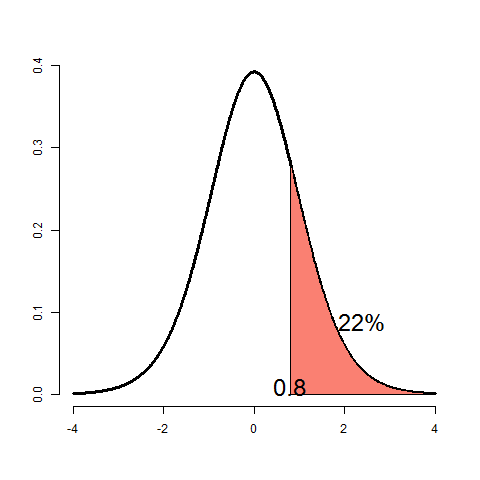
\includegraphics[width=.9\linewidth]{figure3.png}

\begin{itemize}
\item By reporting P-value the reader can perform hypothesis tests he or
  she choses.
\item 2-sided hypothesis is to double smaller of 2-sided P-values
\item Don't just report P-values give confidence intervals
\end{itemize}
\begin{itemize}

\item P-Values Limitations
\label{sec-1-1-3-1}%
\begin{itemize}
\item P-Values only consider significane unlike CIs
\item P-values only measure evidence for NULL not the Alternative
\item Frequently misinterpretted. /Prob. of attaining the value or more
  extreme in favor of the alternative hypothesis when the calculation
  is done under the NULL hypothesis./
\end{itemize}
 
\end{itemize} % ends low level
\subsection{POWER}
\label{sec-1-2}
\subsubsection{What is it}
\label{sec-1-2-1}

\begin{itemize}
\item Probability of rejecting NULL when it is false labeled $\beta$
\item 1- B is Power
\item Consider RDI example
\end{itemize}

$$P\left(\frac{\bar X - 30}{s /\sqrt{n}} > t_{1-\alpha,n-1} ~|~ \mu = \mu_a \right)$$

\begin{itemize}
\item note the function is specific to $\mu$$_a$
\item NOTE as $\mu$$_a$ approaches 30, the power approaches $\alpha$.
\item YOU have to know the value under the alternative you want to plug in
\end{itemize}
\subsubsection{How to calculate it}
\label{sec-1-2-2}

\begin{itemize}
\item Assume that n is large and the we know $\alpha$
\item notice s is replaced by $\sigma$
\item no longer a z-statistic because we are considering an alternative
  hypothesis.
\item Adding and subtracting the mean under the alternative converts it
  to z-statistic.
\end{itemize}

$$1 -\beta  = $$
$$P\left(\frac{\bar X - 30}{\sigma /\sqrt{n}} > z_{1-\alpha} ~|~ \mu = \mu_a \right)$$
$$ =  P\left(\frac{\bar X - \mu_a + \mu_a - 30}{\sigma /\sqrt{n}} > z_{1-\alpha} ~|~ \mu = \mu_a \right)$$
$$ =  P\left(\frac{\bar X - \mu_a}{\sigma /\sqrt{n}} > z_{1-\alpha} - \frac{\mu_a - 30}{\sigma /\sqrt{n}} ~|~ \mu = \mu_a \right)$$
$$ =  P\left(Z > z_{1-\alpha} - \frac{\mu_a - 30}{\sigma /\sqrt{n}}
~|~ \mu = \mu_a \right)$$

\begin{itemize}
\item Suppose we want to detect increase of 2 events per hour
  above 30. Assume normality and the sample will have $\sigma$
  = 4. Sample size is 16:
\item $Z_{1-\alpha} = 1.645$ and
\end{itemize}
$\frac{\mu_a - 30}{\sigma /\sqrt{n}} = 2 / (4 /\sqrt{16}) = 2$ 

\begin{itemize}
\item $P(Z > 1.645 - 2) = P(Z > -0.355) = 64\%$
\item only gets better as difference gets better than 2.
\end{itemize}
\begin{itemize}

\item Given Power what sample size?
\label{sec-1-2-2-1}%
\begin{itemize}
\item Suppose we want power of 0.8
\end{itemize}
$$0.80 = P\left(Z > z_{1-\alpha} - \frac{\mu_a - 30}{\sigma /\sqrt{n}}
~|~ \mu = \mu_a \right)$$

\begin{itemize}
\item set $z_{1-\alpha} - \frac{\mu_a - 30}{\sigma /\sqrt{n}} = z_{0.20}$
  and solve for $n$
\item done at phase of study design
\item The calculation is similiar when $\mu$ < $\mu$$_0$
\item when $\mu$ $\ne$ \textbackslash{} m$_0$
\item pick 1-sided but use $\alpha$/2 it is \emph{right enough} it omits some of
  the probability (that is small enough to be irrelivant).
\item Power goes up as $\alpha$ gets larger - under court of law example
  the odds of convicting an innocent person goes up as the
  probability of convicting a guilty person goes up.
\item difference between NULL and ALTERNATE gets big - power goes up
\item sample size goes up, your power goes up
\end{itemize}

\end{itemize} % ends low level
\subsubsection{T-test}
\label{sec-1-2-3}

\begin{itemize}
\item Power for T-test is more complicated.
\item the power is:
    $$ P\left(\frac{\bar X - 30}{S /\sqrt{n}} > t_{1-\alpha, n-1} ~|~ \mu = \mu_a \right)   $$
\item Notice that this is equal to:
\end{itemize}

$$ = P\left(\sqrt{n}(\bar X - 30) > t_{1 - \alpha, n-1} S ~|~ \mu = \mu_a \right)    $$

$$ =P\left(\frac{\sqrt{n}(\bar X - 30)}{\sigma}   > t_{1-\alpha, n-1} \frac{S}{\sigma} ~|~ \mu = \mu_a \right) $$

\begin{itemize}
\item Continued - how can do with tools we have:
\end{itemize}

$$  P\left(\frac{\sqrt{n}(\bar X - \mu_a)}{\sigma} + \frac{\sqrt{n}(\mu_a - 30)}{\sigma} > \frac{t_{1-\alpha, n-1}}{\sqrt{n-1}}\times \sqrt{\frac{(n-1) S^2}{\sigma^2}} \right)$$

\begin{itemize}
\item which equal to:
\end{itemize}

$$P\left(Z + \frac{\sqrt{n}(\mu_a - 30)}{\sigma} >  \frac{t_{1 - \alpha, n-1}}{\sqrt{n-1}} \sqrt{\chi^2_{n-1}}\right) $$

where Z and X$^2$$_{\mathrm{n-1}}$ are independent standard normal and
chi-squared random variables

\begin{itemize}
\item Easy to solve using Monte Carlo
\end{itemize}
\subsubsection{Using Monte Carlo to do Power}
\label{sec-1-2-4}

\begin{itemize}
\item Simulate pairs of Z and X$^2$ and check which is bigger. If \%1's
  would be approximate probability.
\end{itemize}


\begin{verbatim}
nosim <- 100000
n <- 16
sigma <- 4
mu0 <- 30
mua <- 32
z <- rnorm(nosim)
xsq <- rchisq(nosim, df=15)
t <- qt(0.95,15)
mean(z+sqrt(n) * (mua - mu0)/sigma >
t/sqrt(n-1) * sqrt(xsq))
\end{verbatim}
Returns a vector of 1 (TRUE) and 0 (FALSE). 1 every time left is bigger than right
side of equation. Mean is the proportion (60\%) accuracy: 1/sqrt(100000)
\begin{verbatim}
 0.60762
\end{verbatim}


\begin{verbatim}
x <- power.t.test(n=16, delta=2, sd=4, type="one.sample", alt="one.sided")
print(unlist(x))
\end{verbatim}

\begin{verbatim}
 [1] 0.60474
                                     n                                 delta 
                                  "16"                                   "2" 
                                    sd                             sig.level 
                                   "4"                                "0.05" 
                                 power                           alternative 
                   "0.604032870954103"                           "one.sided" 
                                method 
 "One-sample t test power calculation"
\end{verbatim}

\begin{itemize}
\item Notice that in both cases we gave a \emph{TRUE} mean and standard
  deviation - but we only needed to provided the delta (difference in
  the means divided by the standard deviation).
\end{itemize}
 
\subsection{Hypothesis Testing for comparing 2 means}
\label{sec-1-3}
\subsubsection{Matched Data}
\label{sec-1-3-1}




\begin{verbatim}

diff <- test2 - test1
n <- sum(!is.na(diff)) #49
mean(diff) #2.88
sd(diff) #7.61
testStat <- sqrt(n) * mean(diff) / sd(diff) #2.65
# below works out to be 0.01
2 * pt(abs(testStat), n -1, lower.tail = FALSE)
##uses the R function
t.test(diff)
\end{verbatim}
\begin{itemize}

\item Discussion of matched data
\label{sec-1-3-1-1}%


\item Regression to the mean (or mediocrity)
\label{sec-1-3-1-2}%

\end{itemize} % ends low level
\subsection{Two Sample Tests}
\label{sec-1-4}
\subsubsection{Matched Data}
\label{sec-1-4-1}

\begin{itemize}
\item comparing 2 groups determine if data are paired.
\item observations on same subject
\item compare when match case to control
\item when paired take the difference of the observations.
\item NULL difference is 0
\item Alternative is not 0
\item Test statistic:
\end{itemize}
$$ \frac{\bar{X} - \mu{d0}}{S_d/\sqrt{n_d}} $$
\begin{itemize}
\item $\mu_d0$ is the value under the NULL (typically 0)
\item statistic is a \$t$_{\mathrm{n_d-1}}$ or $z$ statistic
\item $n_d$ is the number of pairs of observations
\item \$SS$_d$ is the standard deviation of difference of the pairs
\item Example from 2 exams (on same students) and testing if there is a
  difference between the means of the other exams?
\item plot the variables (test1 and test2)
\item mean difference plot (Bland and Altman)
\end{itemize}


\begin{verbatim}
diff <- test1 - test2
n <- sum(!is.na(diff))
mean(diff)
sd(diff)
testStat <- sqrt(n) * mean(diff)/sd(diff)
2 * pt(abs(testStat), n-1, lower.tail=FALSE)

#or
t.test(diff)

# p = 0.01 so reject NULL
\end{verbatim}
\begin{itemize}

\item Comments
\label{sec-1-4-1-1}%
\begin{itemize}
\item Ratios more relevant than pair-wise differences?
\item if yes, then do the test on the log-observations
\item when doing plot of var1 and var2 and mean difference plot (Bland
  and Altman plot)
\end{itemize}

\end{itemize} % ends low level
\subsubsection{Regression to the mean}
\label{sec-1-4-2}

\begin{itemize}
\item Francis Galton saw that for matched data high initial observations
  tend to lead to low second observations.
\item sons of tall dads, tend to be a little shorts
\item dads of tall sons tend to be  a little shorter
\item RTM in detail - normalize both scales (so that their means are both
  0 and the sd is 1)
\item The best fitting line is through average and has slope:
\end{itemize}

$$Cor(Test1, Test2) \frac{SD(Test2)}{SD(Test1)} $$

and passes through the point where $x=mean(Test1) y=mean(Test2)$.

\begin{itemize}
\item It also (because we normalized) passes though the origin (0,0) and
  has a slope equal to the $Cor(Test1, Test2)$
\item Cor(Test1, Test2) <1 in general
\item This will be shrunk towards a horizontal line, our expected
  normalized test score for Test2 can be calculated by mutliplying
  Test 1 (normalized) times the Cor(Test1, Test2).
\begin{itemize}
\item Line adjusts for the the regression to the mean for Test 2
   (conditioned on Test 1).
\end{itemize}
\item for Test 1 conditioned on Test 2 we need to multiply Test 2 by
  \$Cor(Test1, Test2)^-1
\item the first case the line is shrunk towards horizontal line, the the
  second case the line is shrunk towards the vertical line
\item Ideal examiner would have little difference between id. line and
  fitted regression
\item More unrelated the exam scores are more pronounced regression to
  the mean
\end{itemize}
\subsubsection{Two Independent groups}
\label{sec-1-4-3}

\begin{itemize}
\item the extention to 2 independent groups
\item $H_0 : \mu_1=\mu_2 vs H_a \mu_1 \ne \mu_2$ or other alternatives
  (> or <)
\item Assuming common variance

 $$
\end{itemize}
\frac{\bar X - \bar Y}{S_p \sqrt{\frac{1}{n_x} +
\frac{1}{n_y}}}
$$
this follows a $t_{n_x + n_y -2}$ distribution under the null
hypothesis with the t-assumptions


\begin{itemize}
\item If assuming common variance is questionable
\end{itemize}
$$
\frac{\bar X - \bar Y}{\sqrt{\frac{S_x^2}{n_x} + \frac{S_y^2}{n_y}}}
$$

follows normal distribution for large values of $n_x$ and
$n_y$. Follows (approx) Student's T if the $X_i$ and $Y_i$ are normally distributed.

\begin{itemize}
\item Appropriate degrees of freedom are
\end{itemize}
$$\frac{(S_x^2 / n_x + S_y^2 / n_y)^2}{(S_x^2 / n_x)^2 / (n_x - 1) + (S_y^2 / n_y)^2 / (n_y - 1)}$$

\begin{itemize}
\item fairly accurate
\item not a lot of intuition as to why it works this way.
\item ok not an integer
\end{itemize}

Final Comments
\begin{itemize}
\item connection between hypothesis test and confidence interval holds
\item don't test for equality of means by comparing confidence intervals
  (definately will reject if they do not overlap, but sometimes
  overlapping CIs will have rejected means)
\item abuse of paired data
\item in general not as powerful
\end{itemize}
\begin{itemize}

\item Example calculation
\label{sec-1-4-3-1}%
\begin{itemize}
\item randomly assign students to two teaching modules
\item same test
\end{itemize}



\begin{center}
\begin{tabular}{lrrr}
 Group    &   N  &  Mean Exam Score  &  SD Exam Score  \\
 Module1  &  50  &             86.9  &           6.07  \\
 Module2  &  50  &             89.8  &           6.06  \\
\end{tabular}
\end{center}



\begin{itemize}
\item pooled SD 6.065 (sqrt of average variances!)
\item test statistic:
\end{itemize}

$$ \frac{89.8-86.8}{6.065\sqrt{\frac{1}{50}+\frac{1}{50}}} $$

\begin{itemize}
\item look over review notes on formal tests of equality of variances
\item CAFO IS NOT A FAN
\item ASSUME NORMALITY IN F-distributions
\item Bootstrap resampling (not F-distribution) for ratio of CI for the
  ratio between variances
\item if not assume not-equality of variances
\item Suppose you have equal numbers of obs. for 2 groups
\item if data are matched (truley), then
\end{itemize}

$$
\sqrt{\frac{\sigma_y^2}{n} + \frac{\sigma_x^2}{n} - 2 \frac{Cov(X, Y)}{n}}
$$

if you ignore matching\ldots{}
$$
\sqrt{\frac{\sigma_y^2}{n} + \frac{\sigma_x^2}{n}}
$$

\begin{itemize}
\item in many cases by ignoring correlation you are inflating standard
  error. In a way you are ignoring information.
\item why not pair all experiments? Sometimes things don't lend
  themselves to paired design - learning effects on tests etc.
\item crossover designs (some take exam1 then exam2 and some exam2 then
  exam1)
\end{itemize}
 
\end{itemize} % ends low level

\end{document}
